\documentclass[a4j,10pt,oneside,openany]{jsbook}
%
\usepackage{amsmath,amssymb}
\usepackage{bm}
\usepackage[dvipdfmx,hiresbb]{graphicx}
\usepackage{ascmac}
\usepackage{makeidx}
\usepackage{float}
\usepackage{wrapfig}
%
%\makeindex
%
\newcommand{\diff}{\mathrm{d}}  %微分記号
\newcommand{\divergence}{\mathrm{div}\,}  %ダイバージェンス
\newcommand{\grad}{\mathrm{grad}\,}  %グラディエント
\newcommand{\rot}{\mathrm{rot}\,}  %ローテーション
\newcommand{\btu}{\bigtriangleup} % triangle mark
\newcommand{\mr}{\mathrm}
%
\setlength{\textwidth}{\fullwidth}
\setlength{\textheight}{44\baselineskip}
\addtolength{\textheight}{\topskip}
\setlength{\voffset}{-0.6in}
%
\title{{\Huge \textbf{Dr.Hongoの数理科学ゼミ 第169問}}\\}
\author{Yuji Hiramatsu}
\date{}
%
%
%
\begin{document}
%
%
\maketitle
%\frontmatter
%\tableofcontents
%
%
%\mainmatter

%\chapter{...}
%\begin{abstract}
%...
%...
%\end{abstract}

{\Huge 169問 解答}

\vspace{3\baselineskip}


{\Large (1)}
\\
\\
\begin{wrapfigure}{r}{25zw}
	\vspace*{-\intextsep}
	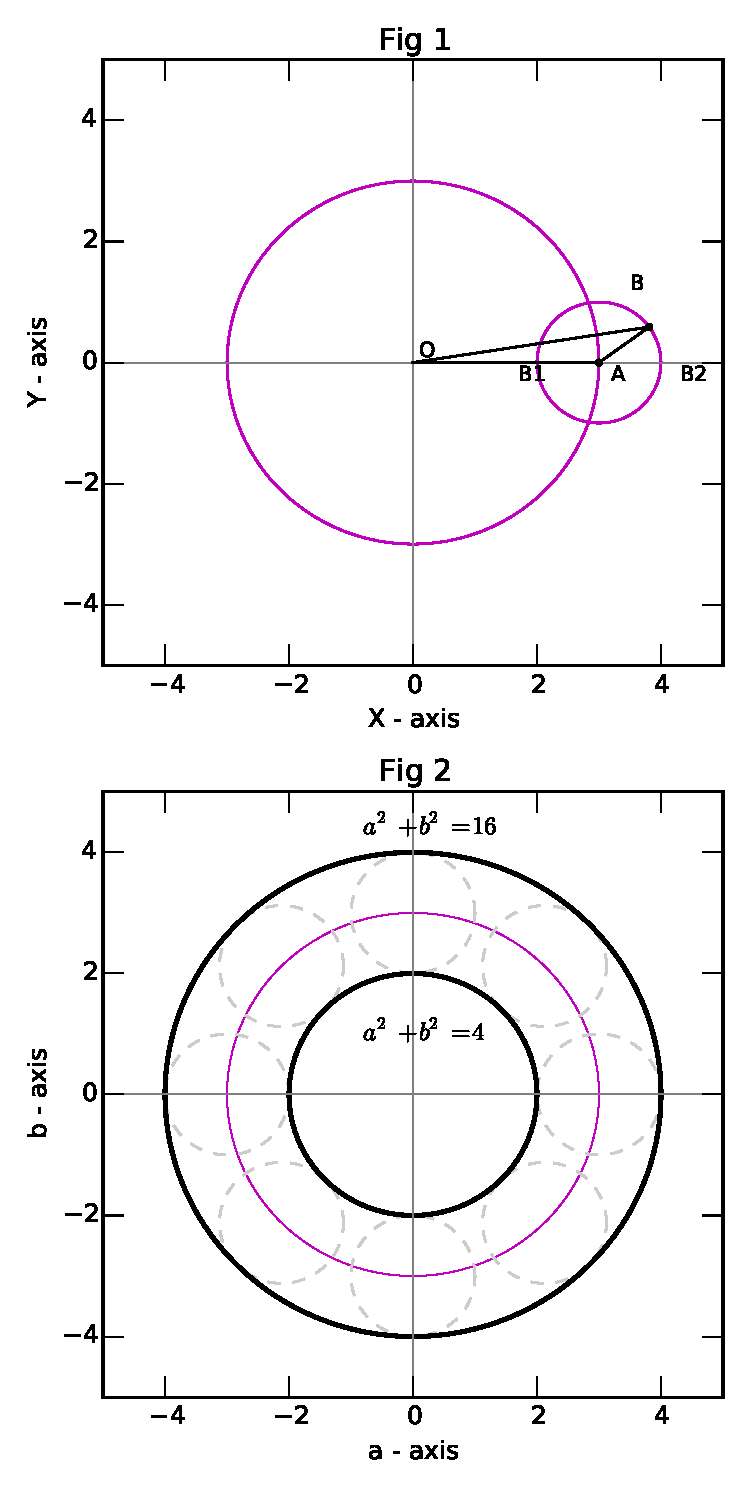
\includegraphics[width=25zw]{fig1.pdf}
	\label{fig}
\end{wrapfigure}
線分OAを$\mathrm{X}$軸としても一般性を失わないので、
題意は、Fig 1のような位置関係となっている。\\
点Bは、点Aを中心とした半径1の円周上を動くことになるので、$0 \leq \angle \mathrm{OAB} \leq \pi$ である。\\
ここで、$\btu \mathrm{OAB}$ に対して、余弦定理を適用すると、\\
\begin{align*}
\mathrm{OB}^2 &= \mathrm{OA}^2 + \mathrm{AB}^2 + 2 \cdot \mathrm{OA} \cdot \mathrm{AB}\cos(\angle \mathrm{OAB}) \\
			&= 3^2 + 1^2 -2\cdot3 \cdot 1 \cdot \cos(\angle \mathrm{OAB})
\end{align*}		
となるので、$0 \leq \angle \mathrm{OAB} \leq \pi$より、\\
\begin{equation*}
2^2 \leq \mathrm{OB}^2 \leq 4^2 \\
\Leftrightarrow \underline{2 \leq \mathrm{OB} \leq 4}
\end{equation*}
{\Large (2)}
\\
\\
題意の式において、$\theta$と$\varphi$が実数解をもつのであれば、Fig 1 における座標軸上で、$(a,b)$は、\\
原点を中心とする半径3の円周上の点を中心とした半径1の円周上を動くこととなる。\\
図示をすると、Fig 2 の太線で表される2つの円$a^2+b^2=4$と$a^2+b^2=16$に囲まれた領域となる。\\
よって、$\underline{4 \leq a^2+b^2 \leq 16}$ \;\;\; (必要条件)\\
次に必要条件を示す。\\
\begin{align*}
a^2+b^2 	&= 9(\sin^2\theta + \cos^2\theta) + (\sin^2\varphi + \cos^2\varphi)+6\cos(\theta-\varphi)\\
		&= 10+6\cos(\theta-\varphi)
\end{align*}
であるので、$4 \leq a^2+b^2 \leq 16$に上式を代入すると、\\
$-1 \leq \cos(\theta-\varphi) \leq 1$を得る。\\
\\
これより、$\theta-\varphi$は任意の実数をとることができるので、\underline{$\theta$及び$\varphi$はそれぞれ任意の実数解をもつ}ことができる。\\
よって、十分条件も示された。
\end{document}











